\chapter{Double pion electroproduction off the proton}
\label{sect:two_pi_prod}
\mbox{}\vspace{-\baselineskip}

%-------------------------------------------------
\section{Differential cross sections and kinematical variables in the experimental data analysis}
\label{sect:cr_sect_exp}


\begin{figure}[htp]
\begin{center}
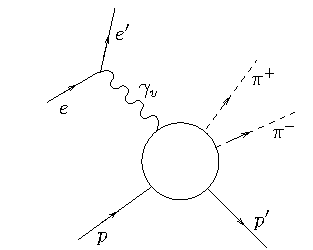
\includegraphics[width=8cm]{pictures/2pi_elprod/2pi_el_prod}
\caption{\small The process of charged double pion electroproduction off the proton.} \label{fig:2pi_el_prod_scheme}
\end{center}
\end{figure}

The process of charged double pion electroproduction off the free proton is schematically shown in Fig.~\ref{fig:2pi_el_prod_scheme}. The cross section of this exclusive reaction is seven-differential and in the one photon exchange approximation connected with the virtual photoproduction cross section via so-called virtual photon flux $\Gamma_{v}$:

\begin{align} \label{cr_s_el}
 \frac{d^{7}\sigma_{e} }{dWdQ^2d^{5}\tau} = \Gamma_{v}\frac{d^{5}\sigma_{v} }{d^{5}\tau},
\end{align}

where $W = \sqrt{(P_{p}+P_{\gamma_v})^2}$ is the invariant mass of the final hadron system, $Q^2 = -(P_{\gamma_v})^2$ the photon virtuality, $P_{\gamma_v} = P_{e} - P_{e'}$ the four-momentum of the virtual photon, $P_{i}$ the four-momentum of the particle $i$, and $d^{5}\tau$ the differential of the five independent variables of the final $\pi^+\pi^-p$ state.

The virtual photon flux $\Gamma_{v}$ in Eq.~\eqref{cr_s_el} is given by

\begin{equation}
\Gamma_{v}(W,Q^2) =
\frac{\alpha}{4\pi}\frac{1}{E_{beam}^{2}m_{p}^{2}}\frac{W(W^{2}-m_{p}^{2})}
{(1-\varepsilon_{T})Q^{2}} \textrm{ ,}
\label{flux}
\end{equation}

where $\alpha$ is the fine structure constant $\left(1/137\right)$, $m_{p}$ the proton mass, $E_{beam}$ the energy of the incoming electron beam, and $\varepsilon_{T}$ the transverse virtual photon polarization, given by

\begin{equation}
\varepsilon_{T} = \left( 1 + 2\left( 1 +
\frac{\nu^{2}}{Q^{2}} \right)
tan^{2}\left(\frac{\theta_{e'}}{2}\right) \right)^{-1} \textrm{ ,}
\label{eq:polarization}
\end{equation}

where $\nu = E_{beam} - E_{e'}$. $E_{e'}$ and $\theta_{e'}$ are the energy of the scattered electron and its polar angle in the lab frame, respectively. 

The conventional choice of five independent variables of the hadron final state is the following:

\begin{itemize}
\item invariant mass of the first pair of the
particles $M_{12}$;
\item invariant mass of the second pair of the
particles $M_{23}$;
\item the first particle's solid angle $\Omega$ = ($\theta$, $\varphi$) (see Fig.~\ref{fig:cr_sec_thetaphi}) and
\item the angle $\alpha$ between two planes: one of
them (plane A) is defined by the three-momenta of
the virtual photon (or initial proton) and the first final hadron, the second
plane (plane B) is defined by the three-momenta of all final hadrons (as shown in  Fig.~\ref{fig:alpha_2nd_set} for the case when $\pi^-$ is chosen as the first particle).
\end{itemize}





%\begin{align}
% d^{5}\tau = dM_{\pi^+p}dM_{\pi^+\pi^-}d\Omega_{\pi^-}d\alpha_{\pi^-},
%\end{align}



\begin{figure}[htp]
\begin{center}
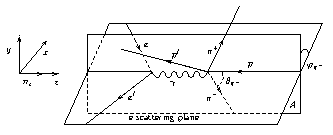
\includegraphics[width=12cm]{pictures/2pi_elprod/thetaphi.pdf}
\caption{\small Polar ($\theta_{\pi^{-}}$) and azimuthal ($\varphi_{\pi^{-}}$) angles of $\pi^{-}$ in the c.m. frame.} \label{fig:cr_sec_thetaphi}
\end{center}
\end{figure}


\begin{figure}[htp]
\begin{center}
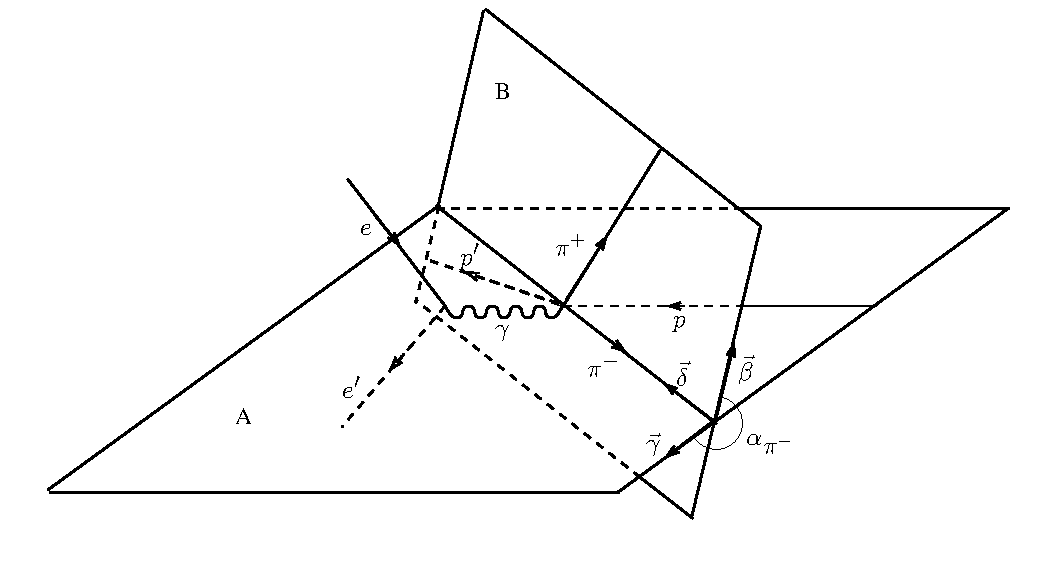
\includegraphics[width=12cm]{pictures/2pi_elprod/alpha1.pdf}
\caption{\small Definition of the angle $\alpha_{\pi^{-}}$ between two planes: the plane B is defined by the three-momenta of all final hadrons, while the plane A is defined by  the three-momenta of $\pi^{-}$ and initial proton. The definitions of  auxiliary vectors $\vec \beta$, $\vec \gamma$, $\vec \delta$ are given in Appendix~\ref{app_a}.} \label{fig:alpha_2nd_set}
\end{center}
\end{figure}



These final hadron variables are defined in the center-of-mass frame of the \textit{virtual photon -- initial proton} system. 




%-------------------------------------------------
%\section{Experimental cross section extraction}

In the experimental data analysis the cross sections are usually obtained in three sets of variables depending on various assignments for the first, second, and third final hadrons:

\begin{enumerate}
\item $\boldsymbol{1st\; - p',\; 2nd \; - \pi^{+},\;3rd - \pi^{-}}$: $M_{p'\pi^{+}}$, $M_{\pi^{+}\pi^{-}}$, $\theta_{p'}$, $\varphi_{p'}$, $\alpha_{(p,p')(\pi^{+},\pi^{-})}$ (or $\alpha_{p'}$);
\item $\boldsymbol{1st\; - \pi^{-},\; 2nd \; - \pi^{+},\;3rd - p'}$: $M_{\pi^{-}\pi^{+}}$, $M_{\pi^{+}p'}$, $\theta_{\pi^{-}}$, $\varphi_{\pi^{-}}$, $\alpha_{(p\pi^{-})(p'\pi^{+})}$ (or $\alpha_{\pi^{-}}$) and
\item $\boldsymbol{1st\; - \pi^{+},\; 2nd \; - \pi^{-},\;3rd - p'}$: $M_{\pi^{+}\pi^{-}}$, $M_{\pi^{-}p'}$, $\theta_{\pi^{+}}$, $\varphi_{\pi^{+}}$, $\alpha_{(p\pi^{+})(p'\pi^{-})}$ (or $\alpha_{\pi^{+}}$).
\end{enumerate}

Limited statistics of the experimental data does not allow to estimate the five-differential cross section with reasonable accuracy. Therefore, the five-differential hadronic cross sections obtained in each bin in $W$ and $Q^2$ are integrated in order to obtain the single-differential cross sections.


The following set of the single-differential cross sections are usually obtained for the second set of variables:
\begin{equation}
\begin{aligned}
\frac{d\sigma}{dM_{\pi^{+}\pi^{-}}} & =
\int\frac{d^{5}\sigma}{d^{5}\tau}d\tau_{M_{\pi^{+}\pi^{-}}}^{4} & \textrm{with}~~~& 
 d\tau_{M_{\pi^{+}\pi^{-}}}^{4} &\!\!\!\!\! =~~ &
dM_{\pi^{+}p}d\Omega_{\pi^{-}}d\alpha_{\pi^{-}}; \\
\frac{d\sigma}{dM_{\pi^{+}p}} & =
\int\frac{d^{5}\sigma}{d^{5}\tau}d\tau_{M_{\pi^{+}p}}^{4}  & \textrm{with}~~~& 
d\tau_{M_{\pi^{+}p}}^{4} &\!\!\!\!\! =~~ &
dM_{\pi^{+}\pi^{-}}d\Omega_{\pi^{-}}d\alpha_{\pi^{-}}; \\
\frac{d\sigma}{d(-cos\theta_{\pi^{-}})} & =
\int\frac{d^{5}\sigma}{d^{5}\tau}d\tau_{\theta_{\pi^{-}}}^{4} & \textrm{with}~~~& 
d\tau_{\theta_{\pi^{-}}}^{4} &\!\!\!\!\! =~~ &
dM_{\pi^{+}\pi^{-}}dM_{\pi^{+}p}d\varphi_{\pi^{-}}d\alpha_{\pi^{-}}; \\
\frac{d\sigma}{\alpha_{\pi^{-}}} & =
\int\frac{d^{5}\sigma}{d^{5}\tau}d\tau_{\alpha_{\pi^{-}}}^{4} & \textrm{with}~~~& 
d\tau_{\alpha_{\pi^{-}}}^{4} &\!\!\!\!\! =~~ &
dM_{\pi^{+}\pi^{-}}dM_{\pi^{+}p}d\Omega_{\pi^{-}};
\end{aligned}
\label{inegr5diff}
\end{equation}
$$
\text{and\,\,\,} d^{5}\tau = dM_{\pi^{+}\pi^{-}}dM_{\pi^{+}p}d\Omega_{\pi^{-}}d\alpha_{\pi^{-}}. 
$$

For the two other sets of variables the single-differential cross sections can be obtained accordingly.


In the actual cross section calculations the integrals in Eq.~\eqref{inegr5diff} are substituted by the respective sums over the five-dimensional  kinematical grid of hadronic cross sections. 

%-------------------------------------------------
\section{Differential cross sections in the model analysis}
\label{sect:cr_sect_model}
After the cross sections have been extracted experimentally they are analyzed with a reaction model with the final goal of extracting resonance electrocouplings and revealing and establishing contributions from different reaction subchannels.  

The phenomenological reaction model, which is used for analyzing double pion cross sections, is the so-called JM ("JLab-Moscow State University") model~\cite{Mokeev:2008iw,Mokeev:2012vsa,Mokeev:2015lda}. The model cross section is parameterized in terms of reaction amplitudes and fitted to the experimental single-differential cross sections by adjusting the free model parameters. In this way for each bin in $W$ and $Q^2$ the model produces the five-differential hadronic cross section that can be suitably used in the EG development. 

Let's briefly sketch the framework in which the JM model operates.

For the case when the incident electron beam is unpolarized the virtual photoproduction cross section in Eq.~\eqref{cr_s_el} can be decomposed in the following way (see \cite{Skorodumina:2016pnb} for details):


 \begin{equation}\label{eq:str_fun_decomp}
\begin{aligned}
 \frac{d^{5}\sigma_{v}}{d^{5}\tau }  = \frac{d^{5}\sigma_{T}}{d^{5}\tau }&+\varepsilon _{L}\frac{d^{5}\sigma_{L}}{d^{5}\tau }+ \varepsilon_{T}\left (\frac{d^{5}\sigma_{TT}}{d^{5}\tau } cos\, 2\varphi + \frac{d^{5}\widetilde{\sigma}_{TT}}{d^{5}\tau } sin\, 2\varphi \right )\\
&+\sqrt{2\varepsilon _{L} ( 1+\varepsilon _{T})}\left (\frac{d^{5}\sigma_{TL}}{d^{5}\tau }cos\, \varphi +\frac{d^{5}\widetilde{\sigma}_{TL}}{d^{5}\tau } sin\, \varphi \right ),
\end{aligned}
\end{equation}



where $\varepsilon_{L} = \frac{Q^2}{\nu^2}\varepsilon_{T}$, $\varepsilon_{T}$ is defined by Eq.~\eqref{eq:polarization}, and $\nu$ is the energy of the virtual photon in the lab frame.

%The derivation of this Eq.~\ref{eq:str_fun_decomp} is given in detail in \cite{Skorodumina:2016pnb}

The functions $\sigma_{T}, \sigma_{L}, \sigma_{TT}, \widetilde{\sigma}_{TT}, \sigma _{TL}, \widetilde{\sigma}_{TL}$  are known as the structure functions of exclusive meson production. They depend on the variables $W$, $Q^2$, and on all of the kinematic variables of the final state, with the exception of the angle $\varphi$. The $\varphi$ dependence is factorized explicitly by the factors $cos\, 2\varphi$, $sin\, 2\varphi$, $cos\, \varphi$, and $sin\, \varphi$. Consequently any structure function, which is differential in $\varphi$, differs from the same function, which if not differential in $\varphi$, only by the integral factor $2\pi$.

If the cross section given by Eq.~\eqref{eq:str_fun_decomp} is integrated over the angle $\varphi$, only the first (transverse) and second (longitudinal) terms remain.

The functions $\widetilde{\sigma}_{TT}$ and $\widetilde{\sigma}_{TL}$ deserve  special attention: they appear in the case of three-hadron final state ($\pi^+ \pi^- p$) but not in single meson electroproduction and they vanish upon integrating over the angle $\alpha$. 


It also needs to be mentioned that the differential cross section in Eq.~\eqref{eq:str_fun_decomp} depends on the beam energy, while the structure functions do not -- the dependence on the beam energy is incorporated into the coefficients in front of them. 

In the limit $Q^2 \rightarrow 0$ that corresponds to the real photoproduction scenario, the coefficients in front of the structure functions force them to vanish, leading $\sigma_{T}$ to be the only remaining term.

As a result of the experimental cross section fitting procedure, the JM model can produce all structure functions from Eq.~\eqref{eq:str_fun_decomp} in the five-dimensional sense. The EG described below is based on these model structure functions.



For the purpose of developing the EG, model structure functions were produced for the second set of variables ($\pi^{-}$ is assumed as the first particle) for those $(W,~Q^2)$ points, where the experimental cross sections are available (see Sect.~\ref{sect:data} for detail). These structure functions are differential in  ($S_{12}$, $S_{23}$, $(-cos\theta_{\pi^{-}})$, $\varphi_{\pi^{-}}$, $\alpha_{\pi^{-}}$), where $S_{12} = M_{12}^{2}$ and $S_{23} = M_{23}^{2}$. 

